% Provenance (never printed): old seconde/premiere S material on the
% atmosphere (water vapour, saturation, cloud formation, the vertical motion
% of air) and enseignement scientifique premiere (water cycle); see
% sources/book2/PROVENANCE.md. Every saturation value, lapse rate,
% condensation level and the lee-wind example are computed in
% figdata/grade-10/clouds.py from the IAPWS saturation curves; the soundings
% are invented examples, said so in the text.
\chapter{Why Clouds Form}\label{ch:g10:why-clouds-form}

On a summer terrace a glass of iced water stands on a table. Within a minute
its outside is covered with tiny drops, and a ring of water spreads at its
foot. The water did not leak through the glass: it came out of the air,
which was cooled where it touched the cold glass. A few hours later,
kilometres above the plain, the same thing happens on a grand scale: bubbles
of warm air rise, cool, and at a certain height the water they carry
appears as the flat-bottomed heaps of white cloud called cumulus. This
chapter explains how much water vapour air can hold, why rising air cools,
at what height clouds form, why some days they stay flat and others they
tower into thunderstorms, and how tiny cloud droplets turn into rain and
snow.

\begin{omfigure}
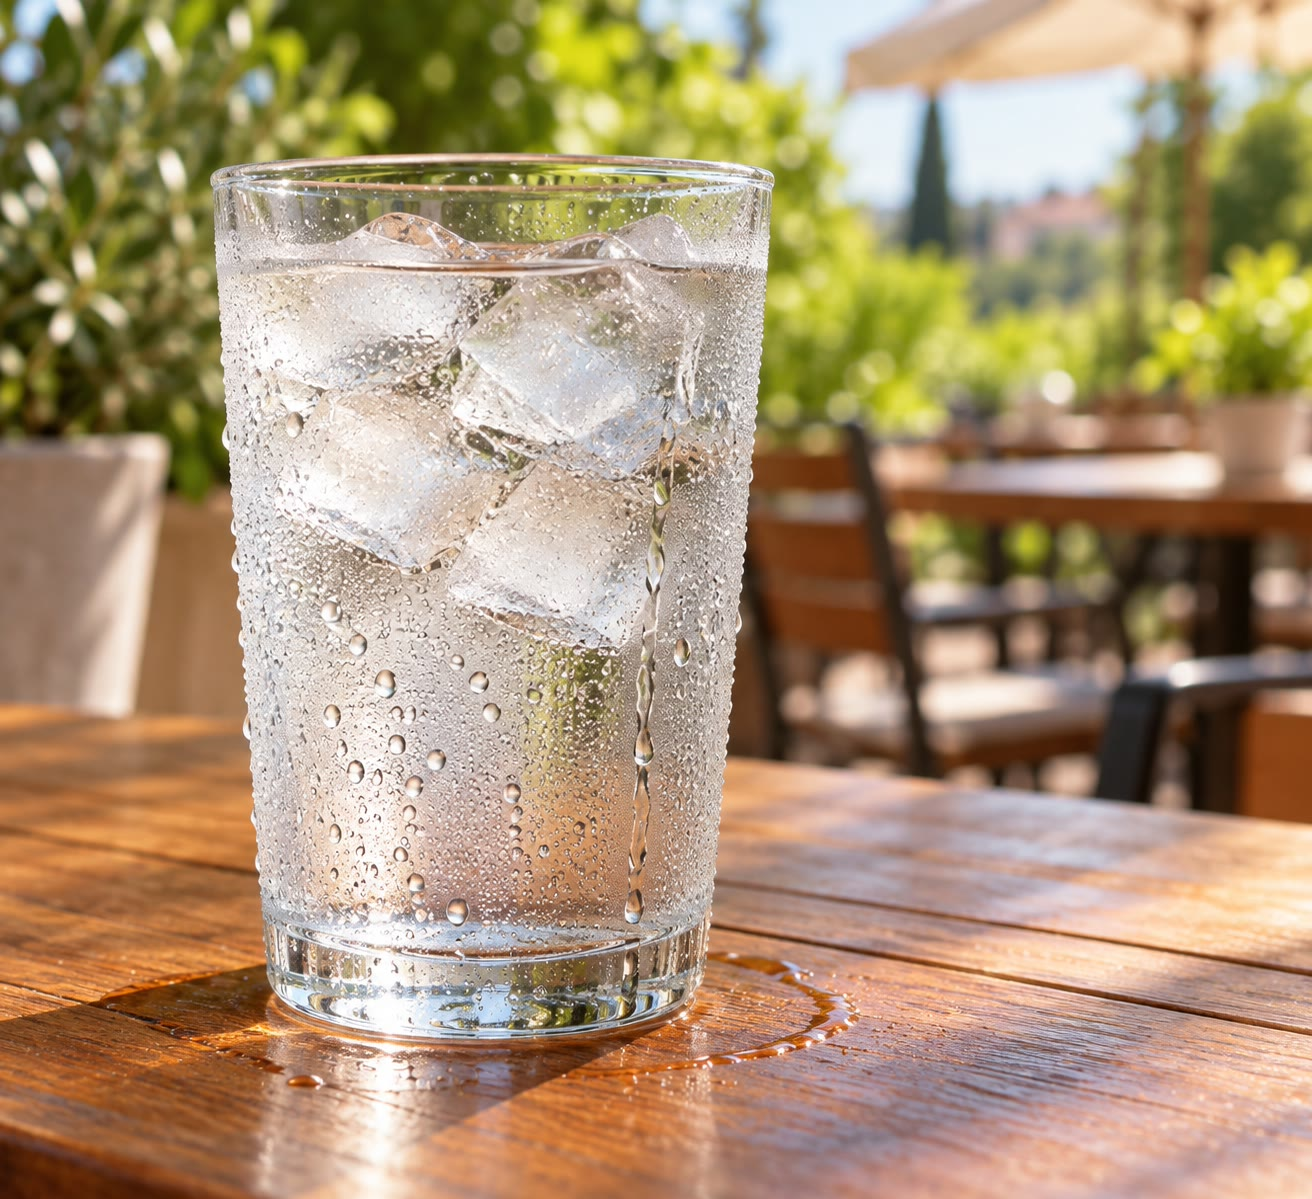
\includegraphics[width=0.5\linewidth]{images/book2/ai/g10-cold-glass.jpg}

{\small A glass of iced water on a summer terrace: drops form on its outside,
where the air touching the glass is cooled.}
\end{omfigure}

\begin{recall}
Clouds are made of tiny droplets of water or crystals of ice; they are
sorted into families by their shape and height, and they give rain, snow
and hail, measured with a rain gauge (Book 1, grade 4). The temperature of
the air falls with height through the lowest layer of the atmosphere, on
average by about \qty{6.5}{\degreeCelsius} per kilometre; this is the
environmental lapse rate, and fronts separate air masses of different
temperatures (Book 1, grade 8). Pressure falls with height (the physics
books). Water evaporates and condenses, and evaporation absorbs \omterm{def:g10:earth-energy-budget:latent-heat}{latent heat}
that condensation gives back (the physics books and
\cref{ch:g10:earth-energy-budget}).
\end{recall}
% ledger: nasa:grc-atmosphere

\section{Water vapour and saturation}

Air always contains some water vapour, an invisible gas. How much it can
contain depends above all on its temperature.

\begin{definition}[Saturation; relative humidity]\label{def:g10:why-clouds-form:humidity}
Air is \emph{saturated}\index{saturation} when it contains the largest mass
of water vapour it can hold at its temperature, its \emph{saturation
content}; any extra vapour condenses into droplets. The \emph{relative
humidity}\index{relative humidity} of air is its content of water vapour
divided by its saturation content at the same temperature and pressure,
expressed as a percentage.
\end{definition}

The water content of air is measured here in grams of vapour per kilogram
of dry air (\unit{g/kg}): a parcel of air that rises or sinks without
gaining or losing water keeps the same content, even as it expands.

\begin{omfigure}
\begin{tikzpicture}
\begin{axis}[omrecord, width=0.88\linewidth, height=6.2cm, xmin=-10, xmax=40,
  ymin=0, ymax=50, xlabel={temperature (\unit{\degreeCelsius})},
  ylabel={saturation content (\unit{g/kg})}, xtick={-10,0,...,40},
  tick label style={font=\small}, label style={font=\small}]
\addplot[omDef!85!black, thick] table[x=T_C, y=ws_gkg] {figdata/out/grade-10-clouds-sat.dat};
\addplot[only marks, mark=*, mark size=1.8pt, omThm!85!black] coordinates {(28,11.37)};
\addplot[only marks, mark=o, mark size=1.8pt, omThm!85!black] coordinates {(16,11.37)};
\draw[->, omThm!85!black, thick] (axis cs:27.2,11.37) -- (axis cs:16.9,11.37);
\node[anchor=north, font=\footnotesize, omThm!85!black] at (axis cs:28,10.6) {air at \qty{28}{\degreeCelsius}};
\node[anchor=south east, font=\footnotesize, omThm!85!black] at (axis cs:15.5,12.2) {dew point};
\node[anchor=south east, font=\footnotesize, omDef!85!black, align=right] at (axis cs:31,34) {above the curve:\\vapour condenses};
\node[anchor=south west, font=\footnotesize, omDef!85!black] at (axis cs:31,2.5) {not saturated};
\node[anchor=north west, font=\footnotesize, omDef!85!black] at (axis cs:34,31.5) {saturation};
\end{axis}
\end{tikzpicture}

{\small The largest mass of water vapour that a kilogram of air can hold,
against temperature, at sea-level pressure (over liquid water; computed from
the international standard for water). Air at \qty{28}{\degreeCelsius}
holding \qty{11.4}{g/kg} (dot) is far from \omterm{def:g10:why-clouds-form:humidity}{saturation}; cooled without losing
water, it becomes \omterm{def:g10:why-clouds-form:humidity}{saturated} at \qty{16}{\degreeCelsius} (circle).}
\end{omfigure}
% ledger: iapws:vapour-pressure, ciaaw:abridged-2024, earth:Mmol, const:R (computed in figdata/grade-10/clouds.py)

The curve rises steeply: \qty{3.8}{g/kg} at \qty{0}{\degreeCelsius},
\qty{14.7}{g/kg} at \qty{20}{\degreeCelsius}, \qty{27.2}{g/kg} at
\qty{30}{\degreeCelsius}. Every \qty{10}{\degreeCelsius} of warming nearly
doubles the water the air can hold. This is why tropical air can carry
torrential rain, and why the air of a polar winter, even \omterm{def:g10:why-clouds-form:humidity}{saturated}, holds
almost nothing.

\begin{definition}[Dew point]\label{def:g10:why-clouds-form:dew-point}
The \emph{dew point}\index{dew point} of air is the temperature to which it
must be cooled, keeping its water content and its pressure, to become
\omterm{def:g10:why-clouds-form:humidity}{saturated}.
\end{definition}

\begin{method}[Relative humidity and dew point from a table]\label{met:g10:why-clouds-form:table}
\begin{enumerate}
  \item Read in the table the \omterm{def:g10:why-clouds-form:humidity}{saturation} content at the air's temperature.
  \item \omterm{def:g10:why-clouds-form:humidity}{Relative humidity}: divide the air's water content by it.
  \item \omterm{def:g10:why-clouds-form:dew-point}{Dew point}: find in the table the temperature whose \omterm{def:g10:why-clouds-form:humidity}{saturation}
        content equals the air's water content.
\end{enumerate}
\end{method}

\begin{example}[A summer morning]\label{ex:g10:why-clouds-form:morning}
% ledger: iapws:vapour-pressure (values computed in figdata/grade-10/clouds.py)
At \qty{20}{\degreeCelsius} the air contains \qty{11.4}{g/kg}. The
\omterm{def:g10:why-clouds-form:humidity}{saturation} content at \qty{20}{\degreeCelsius} is \qty{14.7}{g/kg}, so the
\omterm{def:g10:why-clouds-form:humidity}{relative humidity} is $11.4/14.7 \approx \qty{78}{\percent}$. The \omterm{def:g10:why-clouds-form:humidity}{saturation}
content is \qty{11.4}{g/kg} at \qty{16}{\degreeCelsius}: that is the \omterm{def:g10:why-clouds-form:dew-point}{dew
point}. In the afternoon, the same air warmed to \qty{28}{\degreeCelsius}
(\omterm{def:g10:why-clouds-form:humidity}{saturation} content \qty{24.1}{g/kg}) has a \omterm{def:g10:why-clouds-form:humidity}{relative humidity} of only
\qty{47}{\percent} --- with exactly the same water in it.
\end{example}

The glass of the opening is colder than the \omterm{def:g10:why-clouds-form:dew-point}{dew point} of the air around
it: the air touching it is cooled below its \omterm{def:g10:why-clouds-form:dew-point}{dew point} and gives up water on
the glass. On a clear night, grass and car roofs lose heat by radiating
infrared to the sky and grow colder than the air: dew forms on them, or
frost below \qty{0}{\degreeCelsius}. When a whole layer of air near the
ground cools to its \omterm{def:g10:why-clouds-form:dew-point}{dew point}, droplets form in the air itself: fog.

\begin{omfigure}
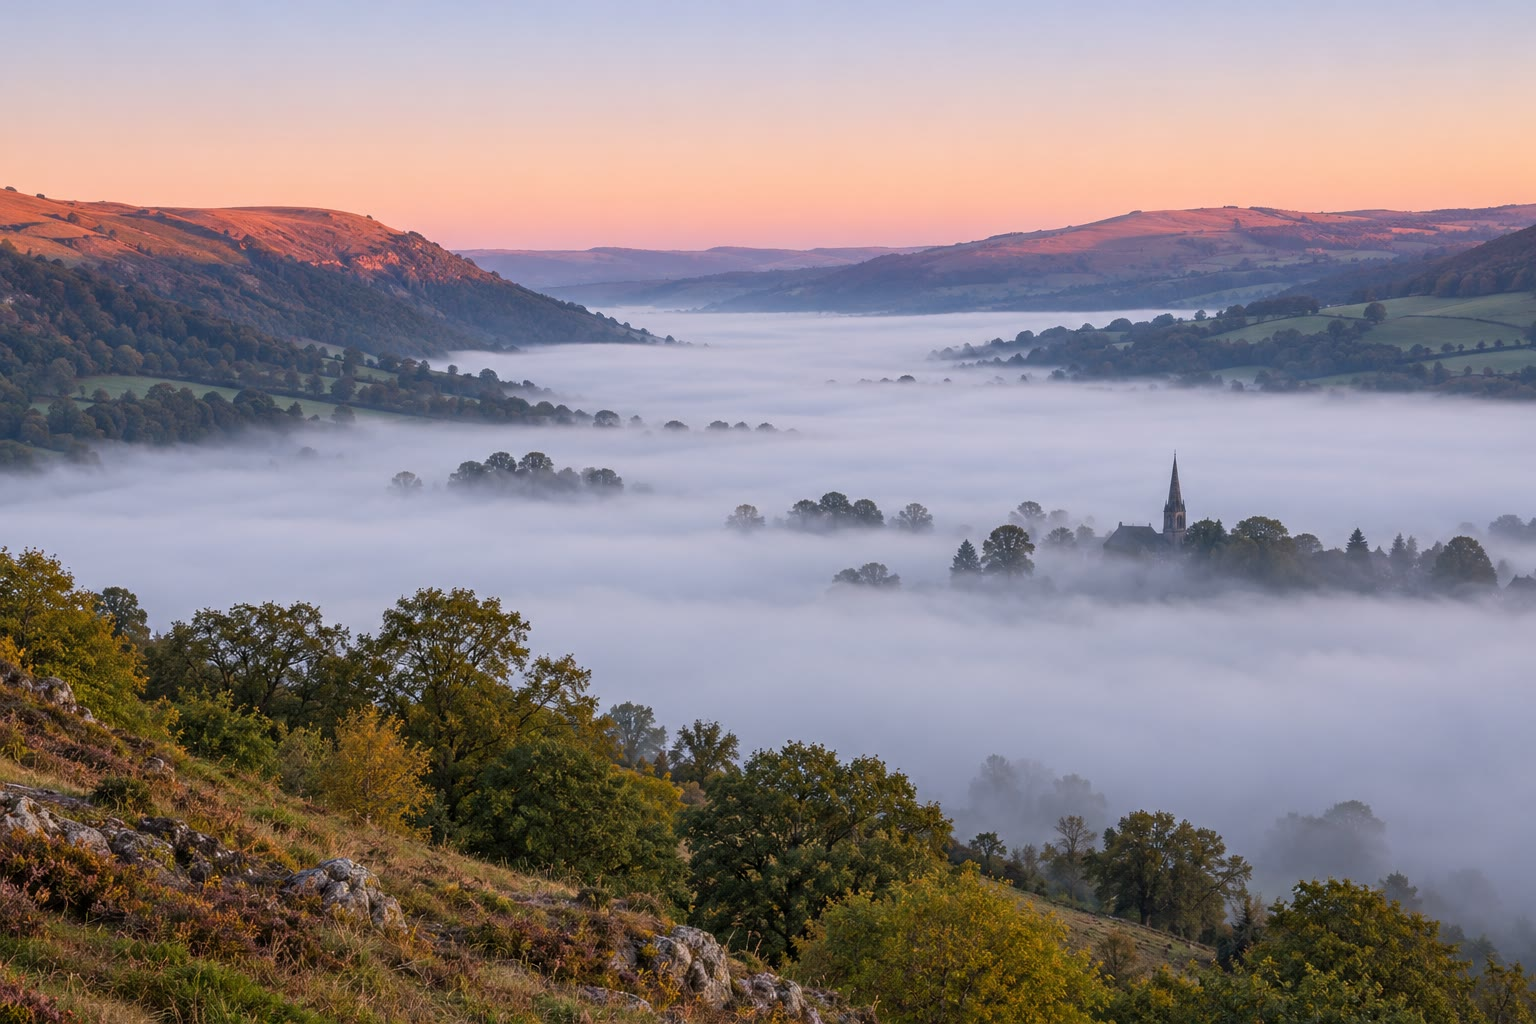
\includegraphics[width=0.75\linewidth]{images/book2/ai/g10-valley-fog.jpg}

{\small Fog filling a valley at dawn. During the clear night the ground
cooled, the cold air drained down into the valley, and there it cooled below
its \omterm{def:g10:why-clouds-form:dew-point}{dew point}.}
\end{omfigure}

\section{Rising air cools}

Most clouds do not form because air touches something cold. They form
because air rises. The pressure falls with height; a parcel of rising air
expands, pushing back the surrounding air, and the energy for this work is
taken from the parcel itself.

\begin{definition}[Adiabatic cooling; dry adiabatic rate]\label{def:g10:why-clouds-form:adiabatic}
\emph{Adiabatic cooling}\index{adiabatic cooling} is the cooling of a
parcel of air that expands without exchanging heat with its surroundings.
The rate at which rising unsaturated air cools in this way is the \emph{dry
adiabatic rate}\index{dry adiabatic rate}, close to
\qty{9.8}{\degreeCelsius} per kilometre of ascent; sinking air warms at the
same rate.
\end{definition}

\begin{proposition}[The dry adiabatic rate]\label{prop:g10:why-clouds-form:dry-rate}
The \omterm{def:g10:why-clouds-form:adiabatic}{dry adiabatic rate} is $g/c_p$, where $g = \qty{9.81}{m/s^2}$ and $c_p
\approx \qty{1005}{J.kg^{-1}.K^{-1}}$ is the energy that warms a kilogram
of air by one degree at constant pressure: $9.81/1005 \approx
\qty{0.0098}{\degreeCelsius/m}$, that is \qty{9.8}{\degreeCelsius/km}.
(Admitted: the proof belongs to the physics books.)
\end{proposition}
% ledger: const:gn, const:R, earth:Mmol (c_p of dry air computed as (7/2)R/M in figdata/grade-10/clouds.py)

The parcel's \omterm{def:g10:why-clouds-form:dew-point}{dew point} also falls as it rises, but slowly: its water content
stays the same, while the drop in pressure makes the vapour a little easier
to saturate. The computation for air near the ground gives about
\qty{1.8}{\degreeCelsius} per kilometre. The parcel's temperature therefore
closes in on its \omterm{def:g10:why-clouds-form:dew-point}{dew point} by about $9.8 - 1.8 = \qty{8}{\degreeCelsius}$
for each kilometre it climbs.
% ledger: iapws:vapour-pressure (dew-point rate computed in figdata/grade-10/clouds.py)

\begin{definition}[Condensation level]\label{def:g10:why-clouds-form:condensation-level}
The \emph{condensation level}\index{condensation level} of a parcel of air
is the height at which, rising, it becomes \omterm{def:g10:why-clouds-form:humidity}{saturated}. Water condenses above
it: the condensation level is the flat base of the clouds that the rising
air forms.
\end{definition}

\begin{proposition}[Height of the condensation level]\label{prop:g10:why-clouds-form:lcl}
Air that rises from the ground with temperature $T$ and \omterm{def:g10:why-clouds-form:dew-point}{dew point} $T_d$
(in \unit{\degreeCelsius}) becomes \omterm{def:g10:why-clouds-form:humidity}{saturated} at about
\[
  z = \frac{T - T_d}{8}\ \text{km} = \qty{125}{m} \times (T - T_d).
\]
\end{proposition}

\begin{proof}
At a height $z$ (in km) the parcel's temperature is $T - 9.8\,z$ and its
\omterm{def:g10:why-clouds-form:dew-point}{dew point} $T_d - 1.8\,z$. It is \omterm{def:g10:why-clouds-form:humidity}{saturated} when they are equal:
$T - 9.8\,z = T_d - 1.8\,z$, so $8\,z = T - T_d$ and $z = (T - T_d)/8$ km.
One eighth of a kilometre is \qty{125}{m}.
\end{proof}

\begin{example}[An afternoon cumulus]\label{ex:g10:why-clouds-form:base}
% ledger: iapws:vapour-pressure (exact ascent computed in figdata/grade-10/clouds.py: 1.51 km)
In the afternoon of \cref{ex:g10:why-clouds-form:morning}, the air at the
ground is at \qty{28}{\degreeCelsius} with a \omterm{def:g10:why-clouds-form:dew-point}{dew point} of
\qty{16}{\degreeCelsius}. Rising bubbles become \omterm{def:g10:why-clouds-form:humidity}{saturated} at
$125 \times 12 = \qty{1500}{m}$: the cumulus have their flat bases about
\qty{1.5}{km} up. In the morning, at \qty{20}{\degreeCelsius}, the same air
would have condensed at only $125 \times 4 = \qty{500}{m}$: cloud bases rise
through the day as the ground warms.
\end{example}

\section{Stable and unstable air}

Whether a rising parcel keeps rising depends on the air around it. A parcel
warmer than its surroundings is lighter than the air it displaces and rises,
like a hot-air balloon; a parcel colder than its surroundings sinks back.

\begin{definition}[Stable air; unstable air]\label{def:g10:why-clouds-form:stability}
Air is \emph{stable}\index{stable air} when a parcel pushed upwards becomes
colder than the air around it, and so sinks back to where it started. It is
\emph{unstable}\index{unstable air} when the parcel becomes warmer than the
air around it and keeps rising on its own.
\end{definition}

The rising parcel cools at the \omterm{def:g10:why-clouds-form:adiabatic}{dry adiabatic rate}, \qty{9.8}{\degreeCelsius}
per kilometre, as long as it is not \omterm{def:g10:why-clouds-form:humidity}{saturated}. Once it is \omterm{def:g10:why-clouds-form:humidity}{saturated} it cools
more slowly: condensation releases \omterm{def:g10:earth-energy-budget:latent-heat}{latent heat} into the parcel. The
computation gives about \qty{4.7}{\degreeCelsius} per kilometre in warm air
near the ground, about \num{5.8} at \qty{0}{\degreeCelsius}, and more in the
cold air higher up, where little water is left to condense; this is the
\omterm{def:g10:why-clouds-form:humidity}{saturated} rate. (Its formula is derived in the university volumes.)
% ledger: nist:water-latent, iapws:vapour-pressure (saturated rates computed in figdata/grade-10/clouds.py)

\begin{method}[Is this air stable?]\label{met:g10:why-clouds-form:stable}
\begin{enumerate}
  \item Find how fast the temperature of the surrounding air falls with
        height (the environmental lapse rate, from a balloon sounding).
  \item Compare it with the rate at which the parcel cools: the dry rate,
        about \qty{9.8}{\degreeCelsius/km}, below its \omterm{def:g10:why-clouds-form:condensation-level}{condensation level};
        the \omterm{def:g10:why-clouds-form:humidity}{saturated} rate, about \qty{5}{\degreeCelsius/km}, above it.
  \item If the surroundings cool more slowly than the parcel, the parcel
        ends up colder: \omterm{def:g10:why-clouds-form:stability}{stable}. If they cool faster, the parcel ends up
        warmer: \omterm{def:g10:why-clouds-form:stability}{unstable}. A layer where the temperature \emph{rises} with
        height is very \omterm{def:g10:why-clouds-form:stability}{stable}: it stops rising air like a lid.
\end{enumerate}
\end{method}

With the average lapse of about \qty{6.5}{\degreeCelsius/km}, air is \omterm{def:g10:why-clouds-form:stability}{stable}
as long as it is unsaturated (the parcel cools faster) and \omterm{def:g10:why-clouds-form:stability}{unstable} once it
is \omterm{def:g10:why-clouds-form:humidity}{saturated} (the parcel cools more slowly). Such air is said to
be conditionally \omterm{def:g10:why-clouds-form:stability}{unstable}: it is \omterm{def:g10:why-clouds-form:stability}{stable} unless something lifts it up to
its \omterm{def:g10:why-clouds-form:condensation-level}{condensation level}, and then the cloud grows on its own.

\begin{omfigure}
\begin{tikzpicture}
\begin{axis}[omrecord, width=0.9\linewidth, height=7.6cm, xmin=-30, xmax=36,
  ymin=0, ymax=6, xlabel={temperature (\unit{\degreeCelsius})}, ylabel={height (km)},
  xtick={-30,-20,...,30}, ytick={0,1,...,6},
  legend style={at={(0.02,0.98)}, anchor=north west, font=\footnotesize, draw=black!30, fill=white},
  tick label style={font=\small}, label style={font=\small}]
\fill[omDef!10] (axis cs:-30,1.51) rectangle (axis cs:36,3.96);
\addplot[black!60, thick] table[x=T_C, y=z_km] {figdata/out/grade-10-clouds-envA.dat};
\addlegendentry{sounding A}
\addplot[omProp!90!black, thick, densely dotted] table[x=T_C, y=z_km] {figdata/out/grade-10-clouds-envB.dat};
\addlegendentry{sounding B}
\addplot[omThm!85!black, very thick] table[x=T_C, y=z_km] {figdata/out/grade-10-clouds-parcel.dat};
\addlegendentry{rising parcel}
\addplot[omMeth!85!black, thick, dashed] table[x=Td_C, y=z_km] {figdata/out/grade-10-clouds-dew.dat};
\addlegendentry{its dew point}
\draw[black!50, dashed] (axis cs:-30,1.51) -- (axis cs:36,1.51);
\node[anchor=south west, font=\footnotesize] at (axis cs:-29.5,1.53) {condensation level};
\node[anchor=north east, font=\footnotesize, omDef!80!black] at (axis cs:35.5,3.9) {cloud with A};
\end{axis}
\end{tikzpicture}

{\small A parcel rising from the ground at \qty{28}{\degreeCelsius} with a
\omterm{def:g10:why-clouds-form:dew-point}{dew point} of \qty{16}{\degreeCelsius} (computed): it cools at the dry rate
until its temperature meets its \omterm{def:g10:why-clouds-form:dew-point}{dew point} at \qty{1.5}{km}, then at the
slower \omterm{def:g10:why-clouds-form:humidity}{saturated} rate. Two invented soundings: in A, the parcel is warmer
than its surroundings from \qty{1.5}{km} up to the warm layer near
\qty{4}{km}, and a cumulus grows between them (shaded); in B, warmer air
above the ground keeps the parcel colder than its surroundings everywhere:
\omterm{def:g10:why-clouds-form:stability}{stable air}, no cumulus.}
\end{omfigure}
% ledger: iapws:vapour-pressure, nist:water-latent (parcel computed in figdata/grade-10/clouds.py; soundings invented)

When the air is \omterm{def:g10:why-clouds-form:stability}{stable} and is lifted all the same --- over a mountain, or
along a front --- the clouds that form spread out in flat grey layers:
stratus. When it is \omterm{def:g10:why-clouds-form:stability}{unstable}, the clouds billow upwards in heaps: cumulus,
and, when the instability reaches high enough, the cumulonimbus of
thunderstorms, whose tops spread out in an anvil where they meet the very
\omterm{def:g10:why-clouds-form:stability}{stable air} above the lowest layer of the atmosphere.

\begin{omfigure}
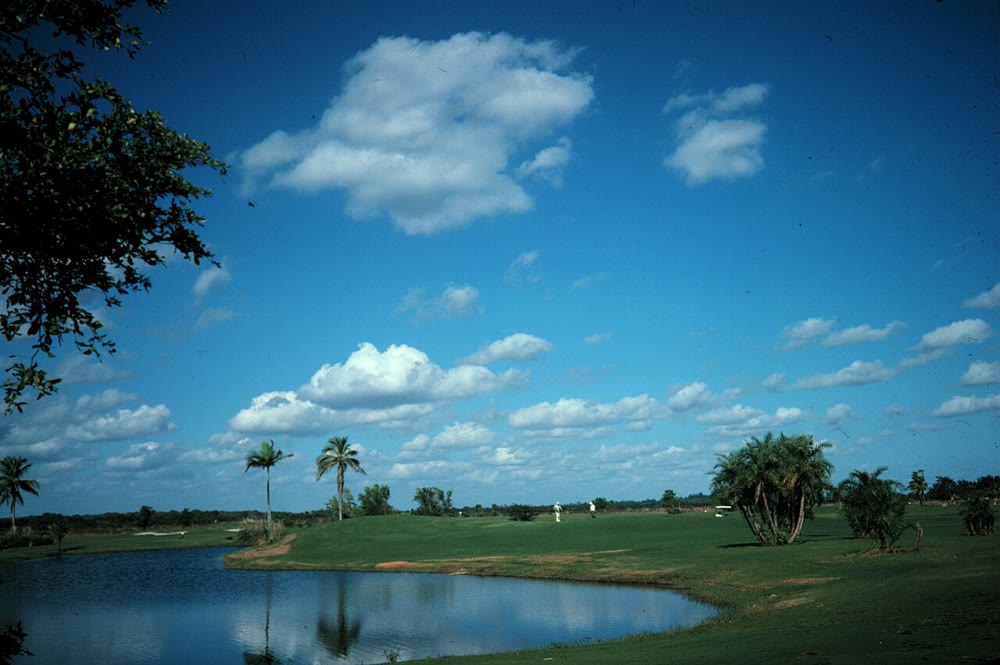
\includegraphics[height=4.5cm]{images/book2/g10-noaa-fair-weather-cumulus.jpg}\hspace{0.6em}%
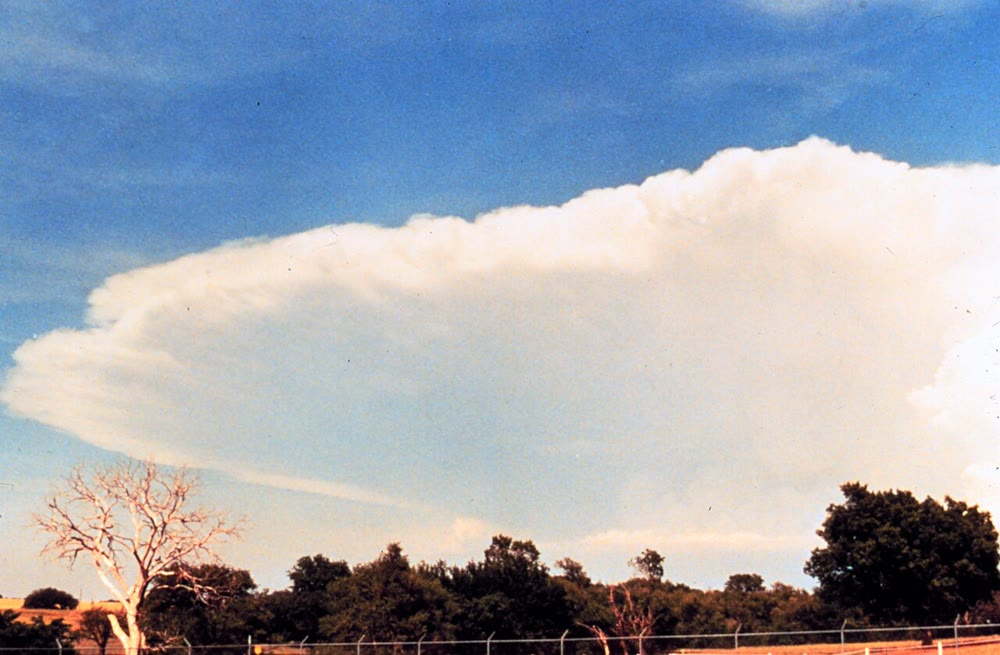
\includegraphics[height=4.5cm]{images/book2/g10-noaa-cumulonimbus-anvil.jpg}

{\small Left: fair-weather cumulus over Florida, with flat bases at their
\omterm{def:g10:why-clouds-form:condensation-level}{condensation level}. Photograph: Ralph F. Kresge, NOAA (public domain).
Right: the anvil of a cumulonimbus in the early stages of a storm.
Photograph: NOAA National Severe Storms Laboratory (public domain).}
\end{omfigure}

\section{Four ways to lift air}

Air rises for four reasons.
\begin{itemize}
  \item \textbf{Heating from below.} On a sunny day the ground warms the air
        above it; bubbles of warm air rise from the hottest patches. These
        give the afternoon cumulus.
  \item \textbf{Mountains.} Wind blowing against a mountain range is forced
        up its slope.
  \item \textbf{Fronts.} Where warm and cold air masses meet, the lighter warm
        air rises over the cold air, or the cold air pushes under it (Book 1,
        grade 8).
  \item \textbf{Convergence.} When winds flow together near the ground, the air
        has nowhere to go but up, as in the belt of rising air near the
        equator and at the centre of a depression.
\end{itemize}

\begin{method}[Following a parcel over a mountain]\label{met:g10:why-clouds-form:mountain}
\begin{enumerate}
  \item Find the \omterm{def:g10:why-clouds-form:condensation-level}{condensation level} with the 125-metre rule; up to it the
        parcel cools at \qty{9.8}{\degreeCelsius/km}.
  \item From there to the crest it cools at the \omterm{def:g10:why-clouds-form:humidity}{saturated} rate; the water
        that condenses falls as rain or snow on the windward side.
  \item Beyond the crest the parcel sinks, unsaturated: it warms at
        \qty{9.8}{\degreeCelsius/km} all the way down.
\end{enumerate}
\end{method}

\begin{example}[The warm dry wind of the lee side]\label{ex:g10:why-clouds-form:lee}
% ledger: iapws:vapour-pressure, nist:water-latent (all values computed in figdata/grade-10/clouds.py)
Air at sea level at \qty{20}{\degreeCelsius}, with a \omterm{def:g10:why-clouds-form:dew-point}{dew point} of
\qty{12}{\degreeCelsius}, is driven over a ridge \qty{2500}{m} high. It
becomes \omterm{def:g10:why-clouds-form:humidity}{saturated} at $125 \times 8 = \qty{1000}{m}$, at about
\qty{10}{\degreeCelsius}. From there to the crest it cools at the \omterm{def:g10:why-clouds-form:humidity}{saturated}
rate, to about \qty{2}{\degreeCelsius}, and loses as rain about a third of
its water (from \num{8.7} to \qty{6.0}{g/kg}). Coming down the other side
it warms at the dry rate over \qty{2.5}{km}: it reaches the plain at about
\qty{27}{\degreeCelsius}, seven degrees warmer than it started, with a
\omterm{def:g10:why-clouds-form:humidity}{relative humidity} of about \qty{27}{\percent}. Such warm, dry winds blow in
the lee of many mountain ranges.
\end{example}

\begin{omfigure}
\begin{tikzpicture}[font=\footnotesize, >={Stealth[length=2mm]}]
  \fill[omExo!30] (0,0) -- (3.5,0.3) -- (6,3.0) -- (8.5,0.3) -- (12,0) -- (12,-0.25) -- (0,-0.25) -- cycle;
  \draw[thick, black!70] (0,0) -- (3.5,0.3) -- (6,3.0) -- (8.5,0.3) -- (12,0);
  \draw[black!40, dashed] (0,1.2) -- (4.6,1.2);
  \node[anchor=south west, black!60, align=left] at (0.1,1.22) {condensation\\level, \qty{1000}{m}};
  \foreach \x in {3.62,3.86,4.1} \draw[omDef!60] (\x,1.2) -- (\x-0.06,{0.3+(\x-0.06-3.5)*1.08+0.04});
  \pic[scale=1.1, transform shape] at (4.6,1.22) {puffycloud};
  \pic[scale=0.9, transform shape] at (5.0,2.2) {puffycloud};
  \draw[->, thick, omDef!80!black] (0.2,0.25) -- (2.8,0.5) .. controls (3.6,0.75) .. (4.4,1.7) -- (5.4,2.9) .. controls (5.8,3.4) and (6.2,3.4) .. (6.6,2.9) -- (7.6,1.7) .. controls (8.4,0.75) .. (9.2,0.5) -- (11.8,0.25);
  \node[anchor=east, align=right] at (3.4,2.15) {\qty{10}{\degreeCelsius}, saturated};
  \node[anchor=south, align=center] at (6.0,3.45) {crest \qty{2500}{m}: \qty{2}{\degreeCelsius}};
  \node[anchor=west, align=left] at (7.75,2.1) {sinks and warms\\at \qty{9.8}{\degreeCelsius/km}};
  \node[anchor=north, align=center] at (1.0,-0.3) {\qty{20}{\degreeCelsius}\\dew point \qty{12}{\degreeCelsius}};
  \node[anchor=north, align=center] at (11.0,-0.3) {\qty{27}{\degreeCelsius}\\dew point \qty{6}{\degreeCelsius}};
  \node[anchor=north, black!60] at (4.0,-0.3) {windward: rain};
  \node[anchor=north, black!60] at (8.2,-0.3) {lee: dry};
\end{tikzpicture}

{\small A parcel of air crossing a mountain ridge (temperatures computed;
vertical scale exaggerated). It cools at the dry rate up to its \omterm{def:g10:why-clouds-form:condensation-level}{condensation
level}, at the slower \omterm{def:g10:why-clouds-form:humidity}{saturated} rate above it, losing water as rain, and warms
at the dry rate all the way down the lee side.}
\end{omfigure}

\section{From droplets to rain and snow}

Water vapour does not condense easily in perfectly clean air. Droplets form
on specks of matter.

\begin{definition}[Condensation nucleus]\label{def:g10:why-clouds-form:nucleus}
A \emph{condensation nucleus}\index{condensation nucleus} is a tiny particle
suspended in the air --- a grain of sea salt, dust, smoke or soot --- on
which water vapour condenses to form a cloud droplet.
\end{definition}

A typical nucleus measures about \qty{0.0002}{mm}, a cloud droplet about
\qty{0.02}{mm}, a drop of drizzle \qty{0.5}{mm} and a raindrop about
\qty{2}{mm}. A raindrop is a hundred times wider than a cloud droplet, so its
volume is $100^3$ times larger: a million cloud droplets make one raindrop. Cloud droplets are so small that the slightest updraught keeps
them aloft; for rain to fall, droplets must grow a hundred-fold.
% ledger: jpl:drop-sizes

\begin{omfigure}
\begin{tikzpicture}
\begin{axis}[width=0.9\linewidth, height=3.4cm, xmode=log, xmin=1e-4, xmax=10,
  ymin=0, ymax=1, axis y line=none, axis x line*=bottom,
  xlabel={diameter (mm), logarithmic scale}, tick label style={font=\small},
  label style={font=\small}, clip=false]
\addplot[only marks, mark=*, omDef!85!black, mark size=2.5pt] coordinates {(0.0002,0.3) (0.02,0.3) (0.5,0.3) (2,0.3)};
\node[anchor=south, font=\footnotesize, align=center] at (axis cs:0.0002,0.42) {condensation\\nucleus};
\node[anchor=south, font=\footnotesize, align=center] at (axis cs:0.02,0.42) {cloud\\droplet};
\node[anchor=south, font=\footnotesize, align=center] at (axis cs:0.5,0.42) {drizzle};
\node[anchor=south, font=\footnotesize, align=center] at (axis cs:2,0.42) {raindrop};
\end{axis}
\end{tikzpicture}

{\small Typical sizes, on a scale where each step is ten times the one
before: each object is about a hundred times wider than the previous one,
apart from drizzle. Data: NASA Jet Propulsion Laboratory.}
\end{omfigure}

Two processes make them grow.

\begin{definition}[Warm-rain process; ice-crystal process]\label{def:g10:why-clouds-form:rain-processes}
In the \emph{warm-rain process}\index{warm-rain process}, the larger
droplets of a cloud fall faster than the small ones, collide with them and
merge, growing as they fall. In the \emph{ice-crystal
process}\index{ice-crystal process}, in the part of a cloud colder than
\qty{0}{\degreeCelsius} where ice crystals and supercooled droplets (liquid
below \qty{0}{\degreeCelsius}) are mixed, the crystals grow by taking the
vapour that the droplets evaporate; they fall as snowflakes, and melt into
raindrops if the air below is warm.
\end{definition}

The \omterm{def:g10:why-clouds-form:rain-processes}{ice-crystal process} works because the \omterm{def:g10:why-clouds-form:humidity}{saturation} content is lower over
ice than over liquid water at the same temperature: at
\qty{-10}{\degreeCelsius} the \omterm{def:g10:why-clouds-form:humidity}{saturation} vapour pressure is \qty{287}{Pa}
over water and \qty{260}{Pa} over ice. Air \omterm{def:g10:why-clouds-form:humidity}{saturated} for the droplets holds
\qty{10}{\percent} more vapour than ice can bear: the vapour condenses on the
crystals, the droplets evaporate to replace it.
% ledger: iapws:vapour-pressure, iapws:melt-subl (computed in figdata/grade-10/clouds.py)

\begin{remark}[Latent heat feeds the storm]\label{rem:g10:why-clouds-form:latent}
Every kilogram of water that condenses in a cloud gives the air about
\qty{2.5}{MJ}, the \omterm{def:g10:earth-energy-budget:latent-heat}{latent heat} taken from the sea or the ground when it
evaporated (\cref{ch:g10:earth-energy-budget}). This heat is what makes the
\omterm{def:g10:why-clouds-form:humidity}{saturated} rate slower than the dry rate and keeps a cumulonimbus rising;
\cref{ch:g10:storms-and-cyclones} follows it into the largest storms.
\end{remark}
% ledger: nist:water-latent

\section{Exercises}

For these exercises, use the \omterm{def:g10:why-clouds-form:humidity}{saturation} contents (in \unit{g/kg}, at
sea-level pressure) of the table below, the dry rate
\qty{9.8}{\degreeCelsius/km}, a dew-point fall of \qty{1.8}{\degreeCelsius/km}
and a \omterm{def:g10:why-clouds-form:humidity}{saturated} rate of \qty{5}{\degreeCelsius/km}.
% ledger: iapws:vapour-pressure (table from figdata/out/grade-10-clouds-sat.dat, rounded)

\begin{center}
\small
\begin{tabular}{l*{11}{c}}
\hline
temperature (\unit{\degreeCelsius}) & 0 & 4 & 8 & 10 & 12 & 14 & 16 & 20 & 24 & 28 & 30 \\
\omterm{def:g10:why-clouds-form:humidity}{saturation} content (\unit{g/kg}) & 3.8 & 5.0 & 6.7 & 7.6 & 8.7 & 10.0 & 11.4 & 14.7 & 18.9 & 24.1 & 27.2 \\
\hline
\end{tabular}
\end{center}

\begin{exercise}[$\star$]\label{exo:g10:why-clouds-form:1}
Define the \omterm{def:g10:why-clouds-form:humidity}{relative humidity} and the \omterm{def:g10:why-clouds-form:dew-point}{dew point} of air.
\end{exercise}

\begin{exercise}[$\star$]\label{exo:g10:why-clouds-form:2}
From the table, give the \omterm{def:g10:why-clouds-form:humidity}{saturation} content at \num{0}, \num{10},
\num{20} and \qty{30}{\degreeCelsius}. By roughly what factor does it grow
for each \qty{10}{\degreeCelsius} of warming?
\end{exercise}

\begin{exercise}[$\star$]\label{exo:g10:why-clouds-form:3}
Air at \qty{24}{\degreeCelsius} contains \qty{10.0}{g/kg} of water vapour.
Find its \omterm{def:g10:why-clouds-form:humidity}{relative humidity} and its \omterm{def:g10:why-clouds-form:dew-point}{dew point}.
\end{exercise}

\begin{exercise}[$\star$]\label{exo:g10:why-clouds-form:4}
Explain why a glass of iced water ``sweats'' in summer, and why it does not
on a very dry winter day indoors.
\end{exercise}

\begin{exercise}[$\star$]\label{exo:g10:why-clouds-form:5}
Name the four ways in which air is made to rise, with an example of each.
\end{exercise}

\begin{exercise}[$\star\star$]\label{exo:g10:why-clouds-form:6}
Using \cref{prop:g10:why-clouds-form:lcl}, find the height of the cloud base
for air at \qty{30}{\degreeCelsius} with a \omterm{def:g10:why-clouds-form:dew-point}{dew point} of
\qty{18}{\degreeCelsius}, and for air at \qty{22}{\degreeCelsius} with a \omterm{def:g10:why-clouds-form:dew-point}{dew
point} of \qty{20}{\degreeCelsius}. Which day is likely to be grey and low?
\end{exercise}

\begin{exercise}[$\star\star$]\label{exo:g10:why-clouds-form:7}
A parcel of unsaturated air leaves the ground at \qty{18}{\degreeCelsius}.
What is its temperature \qty{1}{km} and \qty{2}{km} up, if it stays
unsaturated? Sinking back from \qty{2}{km}, at what temperature does it
reach the ground?
\end{exercise}

\begin{exercise}[$\star\star$]\label{exo:g10:why-clouds-form:8}
A balloon sounding shows the temperature falling by \qty{4}{\degreeCelsius}
per km. Is the air \omterm{def:g10:why-clouds-form:stability}{stable} for an unsaturated parcel? For a \omterm{def:g10:why-clouds-form:humidity}{saturated} one?
On a hot afternoon, the temperature falls by \qty{12}{\degreeCelsius} in the
first kilometre above the ground: what happens to the bubbles of warm air?
\end{exercise}

\begin{exercise}[$\star\star$]\label{exo:g10:why-clouds-form:9}
\omterm{def:g10:why-clouds-form:humidity}{Saturated} air at \qty{20}{\degreeCelsius} is cooled to
\qty{10}{\degreeCelsius}. How many grams of water condense per kilogram of
air? Where does the \omterm{def:g10:earth-energy-budget:latent-heat}{latent heat} released go?
\end{exercise}

\begin{exercise}[$\star\star$]\label{exo:g10:why-clouds-form:10}
How many cloud droplets \qty{0.02}{mm} across make one drop of drizzle
\qty{0.5}{mm} across? One raindrop \qty{2}{mm} across?
\end{exercise}

\begin{exercise}[$\star\star$]\label{exo:g10:why-clouds-form:11}
Explain, step by step, why fog forms in valleys rather than on the hilltops
at dawn after a clear, calm night.
\end{exercise}

\begin{exercise}[$\star\star\star$]\label{exo:g10:why-clouds-form:12}
The dry rate is $a$ and the \omterm{def:g10:why-clouds-form:dew-point}{dew point} falls at the rate $b$ (both in
\unit{\degreeCelsius/km}). Show that the \omterm{def:g10:why-clouds-form:condensation-level}{condensation level} is at
$z = (T - T_d)/(a - b)$. Over a high plateau the \omterm{def:g10:why-clouds-form:dew-point}{dew point} falls at
\qty{1.7}{\degreeCelsius/km}: what does the rule ``\qty{125}{m} per degree''
become?
\end{exercise}

\begin{exercise}[$\star\star\star$]\label{exo:g10:why-clouds-form:13}
Air at sea level at \qty{15}{\degreeCelsius}, with a \omterm{def:g10:why-clouds-form:dew-point}{dew point} of
\qty{11}{\degreeCelsius}, crosses a ridge \qty{2000}{m} high. Following
\cref{met:g10:why-clouds-form:mountain}, find the \omterm{def:g10:why-clouds-form:condensation-level}{condensation level}, the
temperature there, the temperature at the crest, and the temperature at
which the air reaches the plain on the other side.
\end{exercise}

\begin{exercise}[$\star\star\star$]\label{exo:g10:why-clouds-form:14}
At \qty{-20}{\degreeCelsius} the \omterm{def:g10:why-clouds-form:humidity}{saturation} vapour pressure is
\qty{126}{Pa} over water and \qty{103}{Pa} over ice. By what percentage is
air \omterm{def:g10:why-clouds-form:humidity}{saturated} for the droplets oversaturated for the ice? Compare with
\qty{-10}{\degreeCelsius}, and say where in a cloud the \omterm{def:g10:why-clouds-form:rain-processes}{ice-crystal process}
works best.
\end{exercise}

\begin{exercise}[$\star\star\star$]\label{exo:g10:why-clouds-form:15}
The surrounding air cools by \qty{6.5}{\degreeCelsius/km}. A parcel starts at
the same temperature as its surroundings and rises \qty{1}{km}. Compute the
difference between its temperature and that of the surroundings if it is
unsaturated, then if it is \omterm{def:g10:why-clouds-form:humidity}{saturated}. Explain the phrase ``conditionally
\omterm{def:g10:why-clouds-form:stability}{unstable}''.
\end{exercise}

\section{Problem: A Summer Afternoon over the Plain}

\begin{problem}[{Weekend problem --- from the morning humidity to the base
of the afternoon clouds}]
\label{pb:g10:why-clouds-form:1}
% ledger: iapws:vapour-pressure, nist:water-latent (all results computed in figdata/grade-10/clouds.py or from the rounded data below; the sounding is sounding A, invented)
Over a wide plain, on a summer day, the air near the ground contains
\qty{11.4}{g/kg} of water vapour all day. It is at \qty{20}{\degreeCelsius}
in the morning and \qty{28}{\degreeCelsius} in the afternoon. A balloon
sounding (an invented example) gives the temperature of the air above:

\begin{center}
\small
\begin{tabular}{l*{8}{c}}
\hline
height (km) & 0 & 0.5 & 1.0 & 1.5 & 2.5 & 3.5 & 3.6 & 4.0 \\
temperature (\unit{\degreeCelsius}) & 28.0 & 23.1 & 18.2 & 13.4 & 6.9 & 0.4 & $-0.3$ & 1.2 \\
\hline
\end{tabular}
\end{center}

\noindent Use the table of \omterm{def:g10:why-clouds-form:humidity}{saturation} contents and the rates given before
the exercises.

\medskip
\noindent\textbf{Part I --- Humidity.}
\begin{enumerate}
  \item Give the \omterm{def:g10:why-clouds-form:humidity}{saturation} content at \qty{20}{\degreeCelsius}.
  \item Compute the morning \omterm{def:g10:why-clouds-form:humidity}{relative humidity}.
  \item Find the \omterm{def:g10:why-clouds-form:dew-point}{dew point} of the air.
  \item Compute the \omterm{def:g10:why-clouds-form:humidity}{relative humidity} in the afternoon.
  \item Has the air become drier in the afternoon? Explain.
\end{enumerate}

\medskip
\noindent\textbf{Part II --- The night and the dew.}
\begin{enumerate}[resume]
  \item During the night the air near the ground cools. At what temperature
        does dew begin to form?
  \item If the air cools to \qty{12}{\degreeCelsius}, how many grams of
        water per kilogram of air have condensed?
  \item Why does dew form on grass and on car roofs before it forms in the
        air?
\end{enumerate}

\medskip
\noindent\textbf{Part III --- The sounding.}
\begin{enumerate}[resume]
  \item Compute the rate at which the temperature falls between
        \num{0} and \qty{1.5}{km}. Compare it with the dry rate.
  \item Compute it between \num{1.5} and \qty{3.5}{km}.
  \item Is the air between \num{1.5} and \qty{3.5}{km} \omterm{def:g10:why-clouds-form:stability}{stable} for an
        unsaturated parcel? For a \omterm{def:g10:why-clouds-form:humidity}{saturated} one?
  \item What happens between \num{3.6} and \qty{4.0}{km}? What does it do
        to a rising cloud?
\end{enumerate}

\medskip
\noindent\textbf{Part IV --- The cloud base.}
\begin{enumerate}[resume]
  \item Compute the difference between the air's temperature and its \omterm{def:g10:why-clouds-form:dew-point}{dew
        point} at the ground in the afternoon.
  \item Compute the temperature and the \omterm{def:g10:why-clouds-form:dew-point}{dew point} of a bubble of this air
        after it has risen \qty{1}{km}, still unsaturated.
  \item By how much has the difference between the two shrunk? At what rate
        does it shrink?
  \item Show that this rate gives the rule ``\qty{125}{m} per degree''.
  \item What would the cloud base have been in the morning?
  \item Explain why cumulus bases rise during the day.
  \item Write the equation stating that the bubble's temperature equals its
        \omterm{def:g10:why-clouds-form:dew-point}{dew point} at the height $z$ (in km).
  \item Solve it: at what height is the base of the afternoon cumulus?
\end{enumerate}
\end{problem}
